%
% -- Manlio Modugno

\documentclass{beamer} 
\usepackage{eulervm}
%\usepackage{booktabs}
\usepackage{listings}
\usepackage{bold-extra}
\usepackage{cancel}
\usepackage{fancybox}
\usepackage{soul}
\usepackage[english]{babel}
\usepackage[utf8]{inputenc}
\usepackage{hyperref}
\usepackage{amsmath}
%\hypersetup{colorlinks=true,urlcolor=blue}

\newcommand{\codefont}{\fontsize{6}{8}\selectfont}
\lstset{language=[Sharp]C, 
captionpos=b, 
frame=lines,
lineskip= 1pt, %space between lines
basicstyle=\codefont, 
keywordstyle=\color{blue}, 
commentstyle=\color{green}, 
stringstyle=\color{red}, 
numbers=left, 
numberstyle=\tiny, 
stepnumber=2,
numbersep=5pt,
breaklines=true, 
breakatwhitespace=false,
showstringspaces=false,
frame=single,
tabsize=2,
emph={double,bool,int,unsigned,char,true,false,void},
emphstyle=\color{blue},
emph={Assert,Test},
emphstyle=\color{red},
emph={[2]\using,\#define,\#ifdef,\#endif},
emphstyle={[2]\color{blue}}
}


\mode<presentation>
\definecolor{title_color}{RGB}{2,128,181} 
\usetheme{Ilmenau}
\usecolortheme[named=title_color]{structure}
\setbeamercolor{palette quaternary}{use=structure,fg=black,bg=white} %header footer color
\useoutertheme[subsection=false]{smoothbars}
\setbeamercovered{transparent}
\setbeamertemplate{navigation symbols}{}
\setbeamerfont{subsection in toc}{size=\scriptsize}

\title{The Open/Closed Principle}
\author{Manlio Modugno}
\institute[GMTechnologies] 

\date[]{The Open/Closed Principle}

\subject{}

\graphicspath{{img/}}
\pgfdeclareimage[height=0.6cm]{mfg-logo}{img/mfgLogo}
\logo{\pgfuseimage{mfg-logo}}

%
% Content start
%
\begin{document}
\begin{frame}
  \titlepage
\end{frame}

\begin{frame}
  \frametitle{Argomenti Trattati}
  \tableofcontents
\end{frame}


\section{Intro}
\subsection{Intro}
\begin{frame}
  \frametitle{Intro}
  \begin{itemize}
	\item<+-> All systems change during their life cycles!
	\item<+-> OCP helps in writing systems that face change:
	\item<+-> def:\textbf{Software entities (classes, modules, functions, etc.) should be open for extension but closed for modification}
	\item<+-> (i.e.) write code that permits to satisfy changes adding new code not changing the old one (contrast rigidity) 
   \end{itemize}
\end{frame}

\subsection{Description}
\begin{frame}
  \frametitle{Description}
  \begin{itemize}
	\item<+-> \textit{open for extension}: An entity can be extended (i.e. changed) with new behaviors
	\item<+-> \textit{closed for modification}: Extending an entity doesn't require existing code modification (or minimal one...)
   \end{itemize}
\end{frame}

\begin{frame}
  \frametitle{Description}
  \begin{itemize}
	\item<+-> They seems conflicting definitions... how to change behavior of an entity without modifying it? 
	\item<+-> A way, in OOP, is to use abstraction.. think about to an abstract class and all possible derivative implementations.. 
   \end{itemize}
\end{frame}

\begin{frame}
  \frametitle{Description: example}
    example of design not conforming to OCP, if a different version of \textit{Server} comes, we must change \textit{Client} also. \\
    \bigbreak
	\fbox{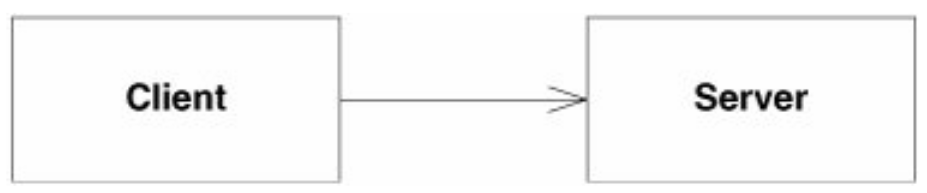
\includegraphics[scale=0.3]{badOcp}}
\end{frame}

\begin{frame}
  \frametitle{Description: example}
    example of design conforming to OCP, if a different version of \textit{Server} comes, \textit{Client} remains unchanged... \\
    \bigbreak
	\fbox{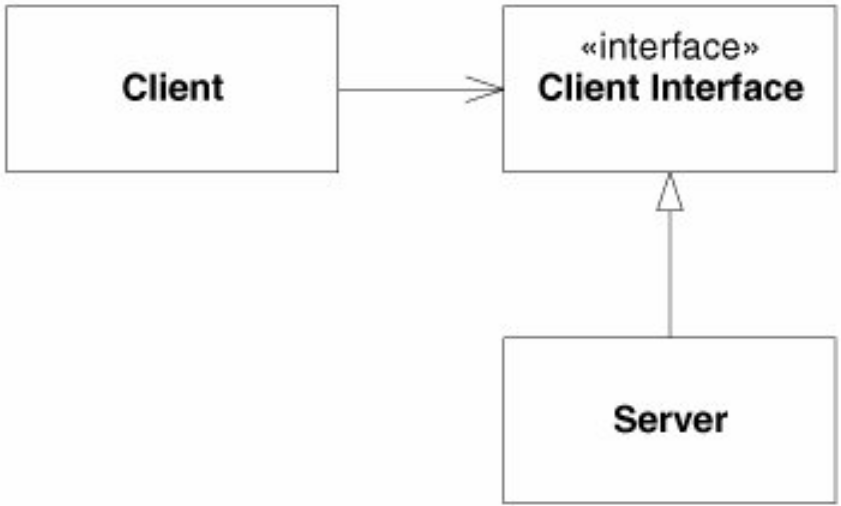
\includegraphics[scale=0.3]{goodOCP}}
\end{frame}

\section{The Shape Application}
\subsection{Shape}
\begin{frame}
  \frametitle{The Shape Application}
  \begin{itemize}
	\item<+-> An application must be able to draw circles and squares on a GUI...
	\item<+-> ..in a particular order using a list..
   \end{itemize}
\end{frame}

\begin{frame}[containsverbatim]
	\frametitle{The Shape Application (procedural approach)}
	A C listing that satisfy (?) \textit{Shape Application}, note that even with non OO languages we can be OCP compliant (see BASH scripting for example...) ! \\
	\begin{lstlisting}
	enum ShapeType {circle, square};
	struct Shape{ShapeType itsType;};
	struct Circle{ShapeType itsType;...};
	void DrawAllShapes(ShapePointer list[], int n){
		int i;
		for (i=0; i<n; i++){
			struct Shape* s = list[i];
			switch (s->itsType){
				case square:
					DrawSquare((struct Square*)s);
				break;
				case circle:
					DrawCircle((struct Circle*)s);
				break;
			}
		}
	}
	\end{lstlisting}
\end{frame}

\begin{frame}
  \frametitle{Shape Application OCP violation}
  \begin{itemize}
	\item<+-> \textit{DrawAllShapes} function It's not closed against new kind of shapes (i.e. a new shape implies a modification in \textit{DrawAllShapes})
	\item<+-> \textit{switch} type used here to distinguish behavior would be used again in other places.. $ \rightarrow $ \textbf{fragility}
	\item<+-> ..``all the same, but a little different''.. never heard it?
	\item<+-> with multiple \textit{switch}, \textit{if/else} a new shape require an hunt in the code to satisfy new requirement $ \rightarrow $ many modifications $ \rightarrow $ \textbf{rigidity}
   \end{itemize}
\end{frame}

\begin{frame}
  \frametitle{Shape Application: problems / consequences}
  \begin{itemize}
	\item<+-> ...can exist pathological situation also, where a particular branch acts exactly as another one, local ``simplification'', and so on...
	\item<+-> in large application a modification like that require a complete redeploy..
	\item<+-> example: in SIS a decoupled modification permits an hot deploy without requiring a jboss restart
	\item<+-> adding a new element is really expensive (do you remember SIS?)
	\item<+-> We can't reuse \textit{DrawAllShapes} without bringing the inner Shapes used $ \rightarrow $ immobility
   \end{itemize}
\end{frame}

\begin{frame}[containsverbatim]
	\frametitle{The Shape Application (OO approach)}
	Here, to add a new shape, all we need to do is to add a new derivative of \textit{Shape} interface, \textit{DrawAllShapes} is closed, its behavior can be extended without modifying it!\\
	\begin{lstlisting}
public interface Shape { void Draw(); }
public class Square : Shape {
	public void Draw() {...}
}
public class Circle : Shape{
	public void Draw(){...}
}
public void DrawAllShapes(IList shapes){
	foreach(Shape shape in shapes){
		shape.Draw();
	}
}
	\end{lstlisting}
\end{frame}

\begin{frame}
  \frametitle{The Shape Application, OO advantages when adding a new Shape}
  \begin{itemize}
	\item<+-> No need to look for places that require changes... $ \rightarrow $ no fragility
	\item<+-> No cascade modifications... $ \rightarrow $ no rigidity
	\item<+-> No obstacles in reusing \textit{DrawAllShapes} in any app.. $ \rightarrow $ no immobility
	\item<+-> ...change is minimized! We modify instance point in the code...
   \end{itemize}
\end{frame}

\begin{frame}
  \frametitle{The Shape Application, new requirement}
  \begin{itemize}
	\item<+-> All \textit{Circle} shapes must be drawn before \textit{Square} ones
	\item<+-> ..\textit{DrawAllShapes} is not closed against this change...
	\item<+-> What?! modeling things with \textit{Shape} and derivatives is so \textbf{natural}..
	\item<+->  ``In general, no matter how "closed" a module is, there will
always be some kind of change against which it is not closed. \textbf{There is no model that is natural to all
contexts} ''
   \end{itemize}
\end{frame}

\subsection{Black/White art}
\begin{frame}
  \frametitle{Black/White art}
  \begin{itemize}
	\item<+-> Since closure cannot be complete, it must be strategic!..
	\item<+-> ..and the best strategy is a probabilistic approach...
	\item<+-> Set design to be close against changes that are more likely to happen..
	\item<+-> Experience and good sense can be useful to determine probability... 
	\item<+-> Conforming to OCP can be expensive.. so should be balanced
   \end{itemize}
\end{frame}

\subsection{Needless Complexity}
\begin{frame}
  \frametitle{Needless Complexity}
  \begin{itemize}
	\item<+-> In order to preempt changes a lot of (useless) abstraction can be introduced...
	\item<+-> We must set the code in a way that can be ready to receive a change.. not force things based on speculation
	\item<+-> ``Fool me once, shame on you. Fool me twice, shame on me.''.. take a first bullet, than change things to avoid the second one..
	\item<+-> ..get feedback on first bullets asap..
   \end{itemize}
\end{frame}

\subsection{Shape Application, new requirement}
\begin{frame}
  \frametitle{Shape Application, new requirement}
  \begin{itemize}
	\item<+-> Got first bullet on order requirement.. how to protect from future changes of \underline{that kind}.. ?
	\item<+-> Closure is based on Abstraction $ \rightarrow $ there's need of some ``ordering abstraction''...
   \end{itemize}
\end{frame}

\begin{frame}[containsverbatim]
	\frametitle{Shape Application, new requirement}
	We can do better ..?\\
	\begin{lstlisting}
public interface Shape: IComparable{ void Draw(); }

public void DrawAllShapes(ArrayList shapes){
shapes.Sort();
foreach(Shape shape in shapes)
shape.Draw();
}

	\end{lstlisting}
\end{frame}

\section{Conclusion}
\begin{frame}
  \frametitle{Conclusion}
  \begin{itemize}
	\item<+-> OCP is a core OO design principle..
	\item<+-> It brings to OO (claimed) benefits: flexibility, reusability and maintainability..
	\item<+-> It can be applied in various context (not only OO lang!)
	\item<+-> Pay attention to \textit{premature abstraction}, introduce it only where frequent changes happen
   \end{itemize}
\end{frame}

\end{document}
